\let\negmedspace\undefined
\let\negthickspace\undefined
\documentclass[journal,12pt,twocolumn]{IEEEtran}
\usepackage{cite}
\usepackage{amsmath,amssymb,amsfonts,amsthm}
\usepackage{algorithmic}
\usepackage{graphicx}
\usepackage{textcomp}
\usepackage{xcolor}
\usepackage{txfonts}
\usepackage{listings}
\usepackage{enumitem}
\usepackage{mathtools}
\usepackage{gensymb}
\usepackage{comment}
\usepackage[breaklinks=true]{hyperref}
\usepackage{tkz-euclide} 
\usepackage{listings}
\usepackage{gvv}                                        
\def\inputGnumericTable{}                                 
\usepackage[latin1]{inputenc}                                
\usepackage{color}                                            
\usepackage{array}                                            
\usepackage{longtable}                                       
\usepackage{calc}                                             
\usepackage{multirow}                                         
\usepackage{hhline}                                           
\usepackage{ifthen}                                           
\usepackage{lscape}

\newtheorem{theorem}{Theorem}[section]
\newtheorem{problem}{Problem}
\newtheorem{proposition}{Proposition}[section]
\newtheorem{lemma}{Lemma}[section]
\newtheorem{corollary}[theorem]{Corollary}
\newtheorem{example}{Example}[section]
\newtheorem{definition}[problem]{Definition}
\newcommand{\BEQA}{\begin{eqnarray}}
\newcommand{\EEQA}{\end{eqnarray}}
\newcommand{\define}{\stackrel{\triangle}{=}}
\theoremstyle{remark}
\newtheorem{rem}{Remark}
\begin{document}

\bibliographystyle{IEEEtran}
\vspace{3cm}

\title{10.5.3.19}
\author{EE23BTECH11065 - prem sagar}
\maketitle
\newpage

\bigskip 

\renewcommand{\thefigure}{\theenumi}
\renewcommand{\thetable}{\theenumi}
\textbf{Question}:\\ 200 logs are stacked in the following manner .20 logs in the bottom row ,19 in the next row ,18 in the row next to it and so on(see Fig 5.5).In how many rows are the 200 logs placed and how many logs are in the top row.
\\\\\textbf{Solution}:
\begin{table}[!ht]
  \centering
  \renewcommand\thetable{1}
  \begin{tabular}{|c|c|c|}
   \hline
   \textbf{Symbol} & \textbf{Value}& \textbf{Description} \\
   \hline
        $ x\brak{0}$ & $20$ & first term of AP\\
        \hline
        d & ${-1}$ & common difference\\
        \hline
        $x\brak{n}$ &  & $\brak{x\brak{0}+nd}u\brak{n}$\\
        \hline
        $y\brak{n}$ & $200$ & \\
        \hline
\end{tabular}

  \caption{input parameters}
  \label{tab:10.5.3.19}
  \end{table}
  \\From \tabref{tab:10.5.3.19}:
\begin{align}
200&=\frac{n+1}{2}\brak{20+20-n}
\\n&=24 \brak{\text{or}} 15
\end{align}
for n=24
\begin{align}
x\brak{24}&=20-24
\\&={-4}
\end{align}
but logs cannot be negative
\\for n=15
\begin{align}
x\brak{15}&=20-15
\\&=5
\end{align}
so 5 logs are there on top row
\\ 15 rows are needed.
\\\begin{figure}[h]
  \renewcommand\thefigure{1}
    \centering
    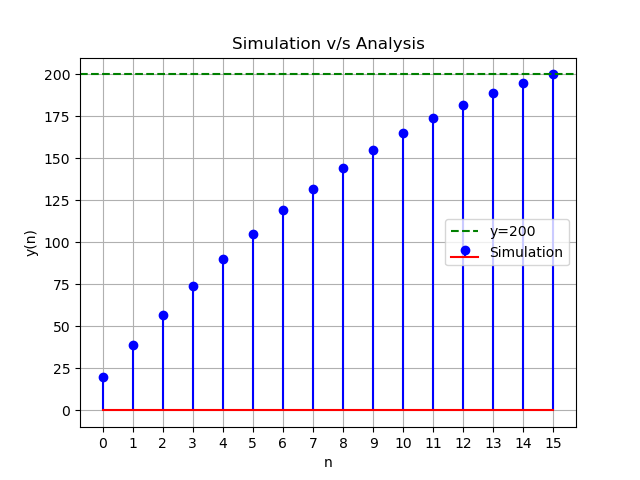
\includegraphics[width=1\linewidth]{/root/assign2/figs/figure_plot.png}
    \caption{plot of y\brak{n} v/s n}
    \label{fig:enter-label}
\end{figure}
\end{document}
